% Options for packages loaded elsewhere
\PassOptionsToPackage{unicode}{hyperref}
\PassOptionsToPackage{hyphens}{url}
%
\documentclass[
]{article}
\usepackage{amsmath,amssymb}
\usepackage{lmodern}
\usepackage{ifxetex,ifluatex}
\ifnum 0\ifxetex 1\fi\ifluatex 1\fi=0 % if pdftex
  \usepackage[T1]{fontenc}
  \usepackage[utf8]{inputenc}
  \usepackage{textcomp} % provide euro and other symbols
\else % if luatex or xetex
  \usepackage{unicode-math}
  \defaultfontfeatures{Scale=MatchLowercase}
  \defaultfontfeatures[\rmfamily]{Ligatures=TeX,Scale=1}
\fi
% Use upquote if available, for straight quotes in verbatim environments
\IfFileExists{upquote.sty}{\usepackage{upquote}}{}
\IfFileExists{microtype.sty}{% use microtype if available
  \usepackage[]{microtype}
  \UseMicrotypeSet[protrusion]{basicmath} % disable protrusion for tt fonts
}{}
\makeatletter
\@ifundefined{KOMAClassName}{% if non-KOMA class
  \IfFileExists{parskip.sty}{%
    \usepackage{parskip}
  }{% else
    \setlength{\parindent}{0pt}
    \setlength{\parskip}{6pt plus 2pt minus 1pt}}
}{% if KOMA class
  \KOMAoptions{parskip=half}}
\makeatother
\usepackage{xcolor}
\IfFileExists{xurl.sty}{\usepackage{xurl}}{} % add URL line breaks if available
\IfFileExists{bookmark.sty}{\usepackage{bookmark}}{\usepackage{hyperref}}
\hypersetup{
  pdftitle={Percentage Delay Rate (Two Quarters): QuickPay (2009-2012)},
  hidelinks,
  pdfcreator={LaTeX via pandoc}}
\urlstyle{same} % disable monospaced font for URLs
\usepackage[margin=1in]{geometry}
\usepackage{graphicx}
\makeatletter
\def\maxwidth{\ifdim\Gin@nat@width>\linewidth\linewidth\else\Gin@nat@width\fi}
\def\maxheight{\ifdim\Gin@nat@height>\textheight\textheight\else\Gin@nat@height\fi}
\makeatother
% Scale images if necessary, so that they will not overflow the page
% margins by default, and it is still possible to overwrite the defaults
% using explicit options in \includegraphics[width, height, ...]{}
\setkeys{Gin}{width=\maxwidth,height=\maxheight,keepaspectratio}
% Set default figure placement to htbp
\makeatletter
\def\fps@figure{htbp}
\makeatother
\setlength{\emergencystretch}{3em} % prevent overfull lines
\providecommand{\tightlist}{%
  \setlength{\itemsep}{0pt}\setlength{\parskip}{0pt}}
\setcounter{secnumdepth}{5}
\usepackage{booktabs,longtable,dcolumn} \usepackage{multirow,array} \usepackage{wrapfig,float} \floatplacement{figure}{H}
\ifluatex
  \usepackage{selnolig}  % disable illegal ligatures
\fi

\title{Percentage Delay Rate (Two Quarters): QuickPay (2009-2012)}
\author{}
\date{\vspace{-2.5em}Nov 16, 2021}

\begin{document}
\maketitle

\hypertarget{delays-over-time}{%
\section{Delays over time}\label{delays-over-time}}

\begin{itemize}
\tightlist
\item
  Sample restricted to projects for which start dates matches the one in
  API

  \begin{itemize}
  \tightlist
  \item
    This is done by using first reported ``action\_date'' and
    ``date\_signed''
  \end{itemize}
\end{itemize}

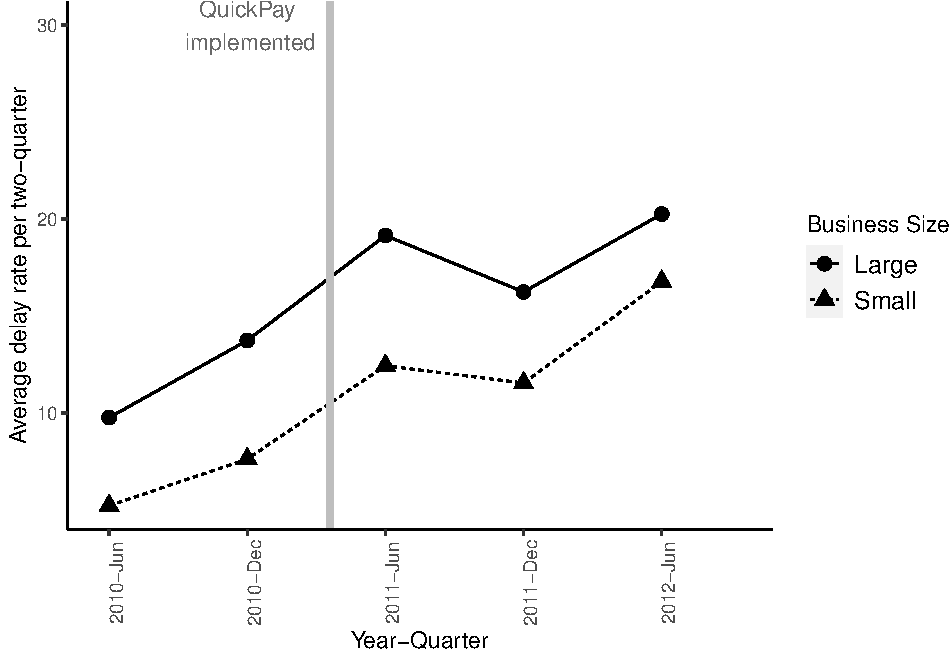
\includegraphics{qp_first_pc_delay_two_quarters_files/figure-latex/plot_pc_delay-1.pdf}

\hypertarget{normalized-delay-rate}{%
\subsection{Normalized delay rate}\label{normalized-delay-rate}}

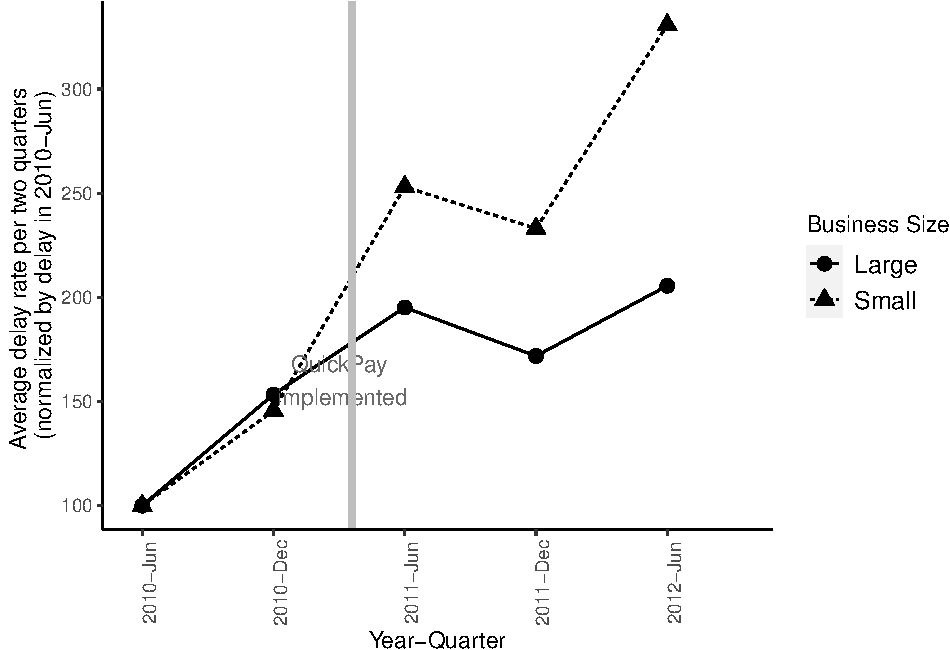
\includegraphics{qp_first_pc_delay_two_quarters_files/figure-latex/normalized_plot-1.pdf}

\hypertarget{full-sample-regressions}{%
\section{Full Sample Regressions}\label{full-sample-regressions}}

\[ \begin{aligned} DelayRate_{it} &=& \alpha+\beta_0 Treat_i + \beta_1 Post_t + \beta_2 (Treat_i \times Post_t)\\
&+&  X_i + (Post_t \times X_i) + \mu_t + \theta_{firm} + \lambda_{task}+ \epsilon_{it}
\end{aligned}\]

\hypertarget{one-quarter}{%
\subsection{One Quarter}\label{one-quarter}}

\begin{table}[H] \centering 
  \caption{Effect of QuickPay on project delay rates} 
  \label{} 
\small 
\begin{tabular}{@{\extracolsep{-2pt}}lccccc} 
\\[-1.8ex]\hline 
\hline \\[-1.8ex] 
\\[-1.8ex] & \multicolumn{5}{c}{$DelayRate_{it}$} \\ 
\\[-1.8ex] & (1) & (2) & (3) & (4) & (5)\\ 
\hline \\[-1.8ex] 
 $Treat_i$ & $-$3.34$^{***}$ & $-$2.72$^{***}$ & $-$2.70$^{***}$ & $-$2.07$^{***}$ & $-$1.81$^{***}$ \\ 
  & (0.15) & (0.15) & (0.15) & (0.15) & (0.35) \\ 
  & & & & & \\ 
 $Post_t$ & 1.02$^{***}$ & $-$1.01$^{***}$ &  &  &  \\ 
  & (0.15) & (0.31) &  &  &  \\ 
  & & & & & \\ 
 $Treat_i \times Post_t$ & 1.34$^{***}$ & 1.62$^{***}$ & 1.62$^{***}$ & 1.33$^{***}$ & 1.51$^{***}$ \\ 
  & (0.19) & (0.20) & (0.20) & (0.19) & (0.21) \\ 
  & & & & & \\ 
 Constant & 8.35$^{***}$ & 16.93$^{***}$ &  &  &  \\ 
  & (0.12) & (0.24) &  &  &  \\ 
  & & & & & \\ 
\hline \\[-1.8ex] 
Duration, Budget, Bids & No & Yes & Yes & Yes & Yes \\ 
$Post_t \times$  (Duration, Budget, Bids) & No & Yes & Yes & Yes & Yes \\ 
Year-Quarter fixed effects & No & No & Yes & Yes & Yes \\ 
Task fixed effects & No & No & No & Yes & Yes \\ 
Contractor fixed effects & No & No & No & No & Yes \\ 
Observations & 287,530 & 263,488 & 263,488 & 263,488 & 263,488 \\ 
R$^{2}$ & 0.004 & 0.05 & 0.06 & 0.09 & 0.17 \\ 
Adjusted R$^{2}$ & 0.004 & 0.05 & 0.06 & 0.09 & 0.12 \\ 
\hline 
\hline \\[-1.8ex] 
\textit{Note:}  & \multicolumn{5}{r}{$^{*}$p$<$0.1; $^{**}$p$<$0.05; $^{***}$p$<$0.01} \\ 
 & \multicolumn{5}{r}{Each observation is a project-quarter.} \\ 
 & \multicolumn{5}{r}{SEs are robust and clustered at the project level.} \\ 
\end{tabular} 
\end{table}

\hypertarget{two-quarters}{%
\subsection{Two-Quarters}\label{two-quarters}}

\begin{table}[H] \centering 
  \caption{Effect of QuickPay on project delay rates} 
  \label{} 
\small 
\begin{tabular}{@{\extracolsep{-2pt}}lccccc} 
\\[-1.8ex]\hline 
\hline \\[-1.8ex] 
\\[-1.8ex] & \multicolumn{5}{c}{$DelayRate_{it}$} \\ 
\\[-1.8ex] & (1) & (2) & (3) & (4) & (5)\\ 
\hline \\[-1.8ex] 
 $Treat_i$ & $-$5.93$^{***}$ & $-$5.10$^{***}$ & $-$5.60$^{***}$ & $-$4.08$^{***}$ & $-$2.62$^{***}$ \\ 
  & (0.27) & (0.27) & (0.26) & (0.26) & (0.65) \\ 
  & & & & & \\ 
 $Post_t$ & 5.53$^{***}$ & 2.30$^{***}$ &  &  &  \\ 
  & (0.29) & (0.54) &  &  &  \\ 
  & & & & & \\ 
 $Treat_i \times Post_t$ & 1.37$^{***}$ & 2.46$^{***}$ & 3.22$^{***}$ & 2.56$^{***}$ & 2.46$^{***}$ \\ 
  & (0.36) & (0.37) & (0.33) & (0.33) & (0.36) \\ 
  & & & & & \\ 
 Constant & 13.00$^{***}$ & 24.09$^{***}$ &  &  &  \\ 
  & (0.23) & (0.41) &  &  &  \\ 
  & & & & & \\ 
\hline \\[-1.8ex] 
Duration, Budget, Bids & No & Yes & Yes & Yes & Yes \\ 
$Post_t \times$  (Duration, Budget, Bids) & No & Yes & Yes & Yes & Yes \\ 
Year-Quarter fixed effects & No & No & Yes & Yes & Yes \\ 
Task fixed effects & No & No & No & Yes & Yes \\ 
Contractor fixed effects & No & No & No & No & Yes \\ 
Observations & 202,125 & 188,575 & 188,575 & 188,575 & 188,575 \\ 
R$^{2}$ & 0.01 & 0.06 & 0.06 & 0.12 & 0.23 \\ 
Adjusted R$^{2}$ & 0.01 & 0.06 & 0.06 & 0.11 & 0.16 \\ 
\hline 
\hline \\[-1.8ex] 
\textit{Note:}  & \multicolumn{5}{r}{$^{*}$p$<$0.1; $^{**}$p$<$0.05; $^{***}$p$<$0.01} \\ 
 & \multicolumn{5}{r}{Each observation is a project-quarter.} \\ 
 & \multicolumn{5}{r}{SEs are robust and clustered at the project level.} \\ 
\end{tabular} 
\end{table}

\hypertarget{truncated-sample-with-positive-delays}{%
\section{Truncated Sample with Positive
Delays}\label{truncated-sample-with-positive-delays}}

\[ \begin{aligned} DelayRate_{it} &=& \alpha+\beta_0 Treat_i + \beta_1 Post_t + \beta_2 (Treat_i \times Post_t)\\
&+&  X_i + (Post_t \times X_i) + \mu_t + \theta_{firm} + \lambda_{task}+ \epsilon_{it}
\end{aligned}\]

\hypertarget{one-quarter-1}{%
\subsection{One Quarter}\label{one-quarter-1}}

\begin{table}[H] \centering 
  \caption{Effect of QuickPay on project delay rates} 
  \label{} 
\small 
\begin{tabular}{@{\extracolsep{-2pt}}lccccc} 
\\[-1.8ex]\hline 
\hline \\[-1.8ex] 
\\[-1.8ex] & \multicolumn{5}{c}{$DelayRate_{it}$} \\ 
\\[-1.8ex] & (1) & (2) & (3) & (4) & (5)\\ 
\hline \\[-1.8ex] 
 $Treat_i$ & $-$9.22$^{***}$ & $-$9.34$^{***}$ & $-$9.38$^{***}$ & $-$7.62$^{***}$ & $-$5.47$^{***}$ \\ 
  & (0.69) & (0.69) & (0.68) & (0.70) & (2.11) \\ 
  & & & & & \\ 
 $Post_t$ & 2.29$^{***}$ & $-$0.51 &  &  &  \\ 
  & (0.54) & (0.78) &  &  &  \\ 
  & & & & & \\ 
 $Treat_i \times Post_t$ & 6.78$^{***}$ & 6.62$^{***}$ & 6.67$^{***}$ & 6.25$^{***}$ & 4.84$^{***}$ \\ 
  & (0.82) & (0.82) & (0.81) & (0.80) & (0.99) \\ 
  & & & & & \\ 
 Constant & 73.51$^{***}$ & 73.36$^{***}$ &  &  &  \\ 
  & (0.45) & (0.61) &  &  &  \\ 
  & & & & & \\ 
\hline \\[-1.8ex] 
Duration, Budget, Bids & No & Yes & Yes & Yes & Yes \\ 
$Post_t \times$  (Duration, Budget, Bids) & No & Yes & Yes & Yes & Yes \\ 
Year-Quarter fixed effects & No & No & Yes & Yes & Yes \\ 
Task fixed effects & No & No & No & Yes & Yes \\ 
Contractor fixed effects & No & No & No & No & Yes \\ 
Observations & 30,138 & 30,130 & 30,130 & 30,130 & 30,130 \\ 
R$^{2}$ & 0.01 & 0.02 & 0.03 & 0.14 & 0.39 \\ 
Adjusted R$^{2}$ & 0.01 & 0.02 & 0.03 & 0.11 & 0.21 \\ 
\hline 
\hline \\[-1.8ex] 
\textit{Note:}  & \multicolumn{5}{r}{$^{*}$p$<$0.1; $^{**}$p$<$0.05; $^{***}$p$<$0.01} \\ 
 & \multicolumn{5}{r}{Each observation is a project-quarter.} \\ 
 & \multicolumn{5}{r}{SEs are robust and clustered at the project level.} \\ 
\end{tabular} 
\end{table}

\hypertarget{two-quarters-1}{%
\subsection{Two Quarters}\label{two-quarters-1}}

\begin{table}[H] \centering 
  \caption{Effect of QuickPay on project delay rates} 
  \label{} 
\small 
\begin{tabular}{@{\extracolsep{-2pt}}lccccc} 
\\[-1.8ex]\hline 
\hline \\[-1.8ex] 
\\[-1.8ex] & \multicolumn{5}{c}{$DelayRate_{it}$} \\ 
\\[-1.8ex] & (1) & (2) & (3) & (4) & (5)\\ 
\hline \\[-1.8ex] 
 $Treat_i$ & $-$17.09$^{***}$ & $-$17.16$^{***}$ & $-$20.72$^{***}$ & $-$16.17$^{***}$ & $-$12.32$^{***}$ \\ 
  & (1.26) & (1.27) & (1.23) & (1.24) & (3.68) \\ 
  & & & & & \\ 
 $Post_t$ & 14.29$^{***}$ & 9.96$^{***}$ &  &  &  \\ 
  & (1.00) & (1.42) &  &  &  \\ 
  & & & & & \\ 
 $Treat_i \times Post_t$ & 12.60$^{***}$ & 12.18$^{***}$ & 17.06$^{***}$ & 14.80$^{***}$ & 11.86$^{***}$ \\ 
  & (1.47) & (1.48) & (1.40) & (1.38) & (1.75) \\ 
  & & & & & \\ 
 Constant & 94.59$^{***}$ & 91.27$^{***}$ &  &  &  \\ 
  & (0.86) & (1.19) &  &  &  \\ 
  & & & & & \\ 
\hline \\[-1.8ex] 
Duration, Budget, Bids & No & Yes & Yes & Yes & Yes \\ 
$Post_t \times$  (Duration, Budget, Bids) & No & Yes & Yes & Yes & Yes \\ 
Year-Quarter fixed effects & No & No & Yes & Yes & Yes \\ 
Task fixed effects & No & No & No & Yes & Yes \\ 
Contractor fixed effects & No & No & No & No & Yes \\ 
Observations & 27,742 & 27,734 & 27,734 & 27,734 & 27,734 \\ 
R$^{2}$ & 0.03 & 0.04 & 0.04 & 0.17 & 0.44 \\ 
Adjusted R$^{2}$ & 0.03 & 0.04 & 0.04 & 0.14 & 0.25 \\ 
\hline 
\hline \\[-1.8ex] 
\textit{Note:}  & \multicolumn{5}{r}{$^{*}$p$<$0.1; $^{**}$p$<$0.05; $^{***}$p$<$0.01} \\ 
 & \multicolumn{5}{r}{Each observation is a project-quarter.} \\ 
 & \multicolumn{5}{r}{SEs are robust and clustered at the project level.} \\ 
\end{tabular} 
\end{table}

\end{document}
